\documentclass[border=12pt]{standalone}
\usepackage{tikz}
\usetikzlibrary{arrows.meta, fit, backgrounds, positioning, calc}
\usepackage{amsmath, amssymb}

\definecolor{Ct}{RGB}{31,88,235}
\definecolor{Cs}{RGB}{205,95,10}
\definecolor{Cm}{RGB}{110,35,160}
\definecolor{Cbgat} {RGB}{237,245,255}
\definecolor{Cbgbsa}{RGB}{255,244,228}

%% ── 3-D feature-map block centred at (#1,#2), colour #3 ─────────────────────
\newcommand{\fmblock}[3]{%
  \pgfmathsetmacro{\cx}{#1}\pgfmathsetmacro{\cy}{#2}%
  \fill[#3!12,draw=#3!75,line width=0.65pt]
    (\cx-1.15,\cy-0.70) rectangle (\cx+1.15,\cy+0.70);
  \fill[#3!22]
    (\cx-1.15,\cy+0.70)--(\cx-0.80,\cy+1.05)--
    (\cx+1.50,\cy+1.05)--(\cx+1.15,\cy+0.70)--cycle;
  \draw[#3!75,line width=0.65pt]
    (\cx-1.15,\cy+0.70)--(\cx-0.80,\cy+1.05)--
    (\cx+1.50,\cy+1.05)--(\cx+1.15,\cy+0.70);
  \fill[#3!8]
    (\cx+1.15,\cy-0.70)--(\cx+1.50,\cy-0.35)--
    (\cx+1.50,\cy+1.05)--(\cx+1.15,\cy+0.70)--cycle;
  \draw[#3!75,line width=0.65pt]
    (\cx+1.15,\cy-0.70)--(\cx+1.50,\cy-0.35)--(\cx+1.50,\cy+1.05)
    (\cx+1.15,\cy-0.70)--(\cx+1.15,\cy+0.70);}

%% ── 3×3 heatmap (cell=0.40, total 1.2×1.2) centred at (#1,#2), colour #3 ───
%% 4th arg: 9 triplets  row/col/intensity  e.g. 0/0/88,0/1/45,...
\newcommand{\heatmap}[4]{%
  \pgfmathsetmacro{\cx}{#1}\pgfmathsetmacro{\cy}{#2}%
  \foreach \ii/\jj/\vv in {#4}{%
    \pgfmathsetmacro{\xl}{\cx-0.60+\jj*0.40}%
    \pgfmathsetmacro{\xr}{\cx-0.60+\jj*0.40+0.40}%
    \pgfmathsetmacro{\yb}{\cy+0.20-\ii*0.40}%
    \pgfmathsetmacro{\yt}{\cy+0.60-\ii*0.40}%
    \fill[#3!\vv](\xl,\yb) rectangle (\xr,\yt);}%
  \draw[#3!45,line width=0.5pt]
    (\cx-0.60,\cy-0.60) rectangle (\cx+0.60,\cy+0.60);
  \foreach \kk in {1,2}{%
    \pgfmathsetmacro{\gx}{\cx-0.60+\kk*0.40}%
    \draw[#3!18,line width=0.22pt](\gx,\cy-0.60)--(\gx,\cy+0.60);
    \pgfmathsetmacro{\gy}{\cy-0.60+\kk*0.40}%
    \draw[#3!18,line width=0.22pt](\cx-0.60,\gy)--(\cx+0.60,\gy);}}

%% ── B×D matrix bar centred at (#1,#2), colour #3 ────────────────────────────
\newcommand{\mmatrix}[3]{%
  \pgfmathsetmacro{\cx}{#1}\pgfmathsetmacro{\cy}{#2}%
  \fill[#3!10,draw=#3!50,line width=0.6pt]
    (\cx-1.30,\cy-0.30) rectangle (\cx+1.30,\cy+0.30);
  \foreach \kk in {1,2,3}{%
    \pgfmathsetmacro{\ry}{\cy-0.30+\kk*0.20}%
    \draw[#3!16,line width=0.3pt](\cx-1.30,\ry)--(\cx+1.30,\ry);}
  \draw[#3!14,line width=0.3pt,dashed]
    (\cx+0.40,\cy-0.30)--(\cx+0.40,\cy+0.30);}

\begin{document}
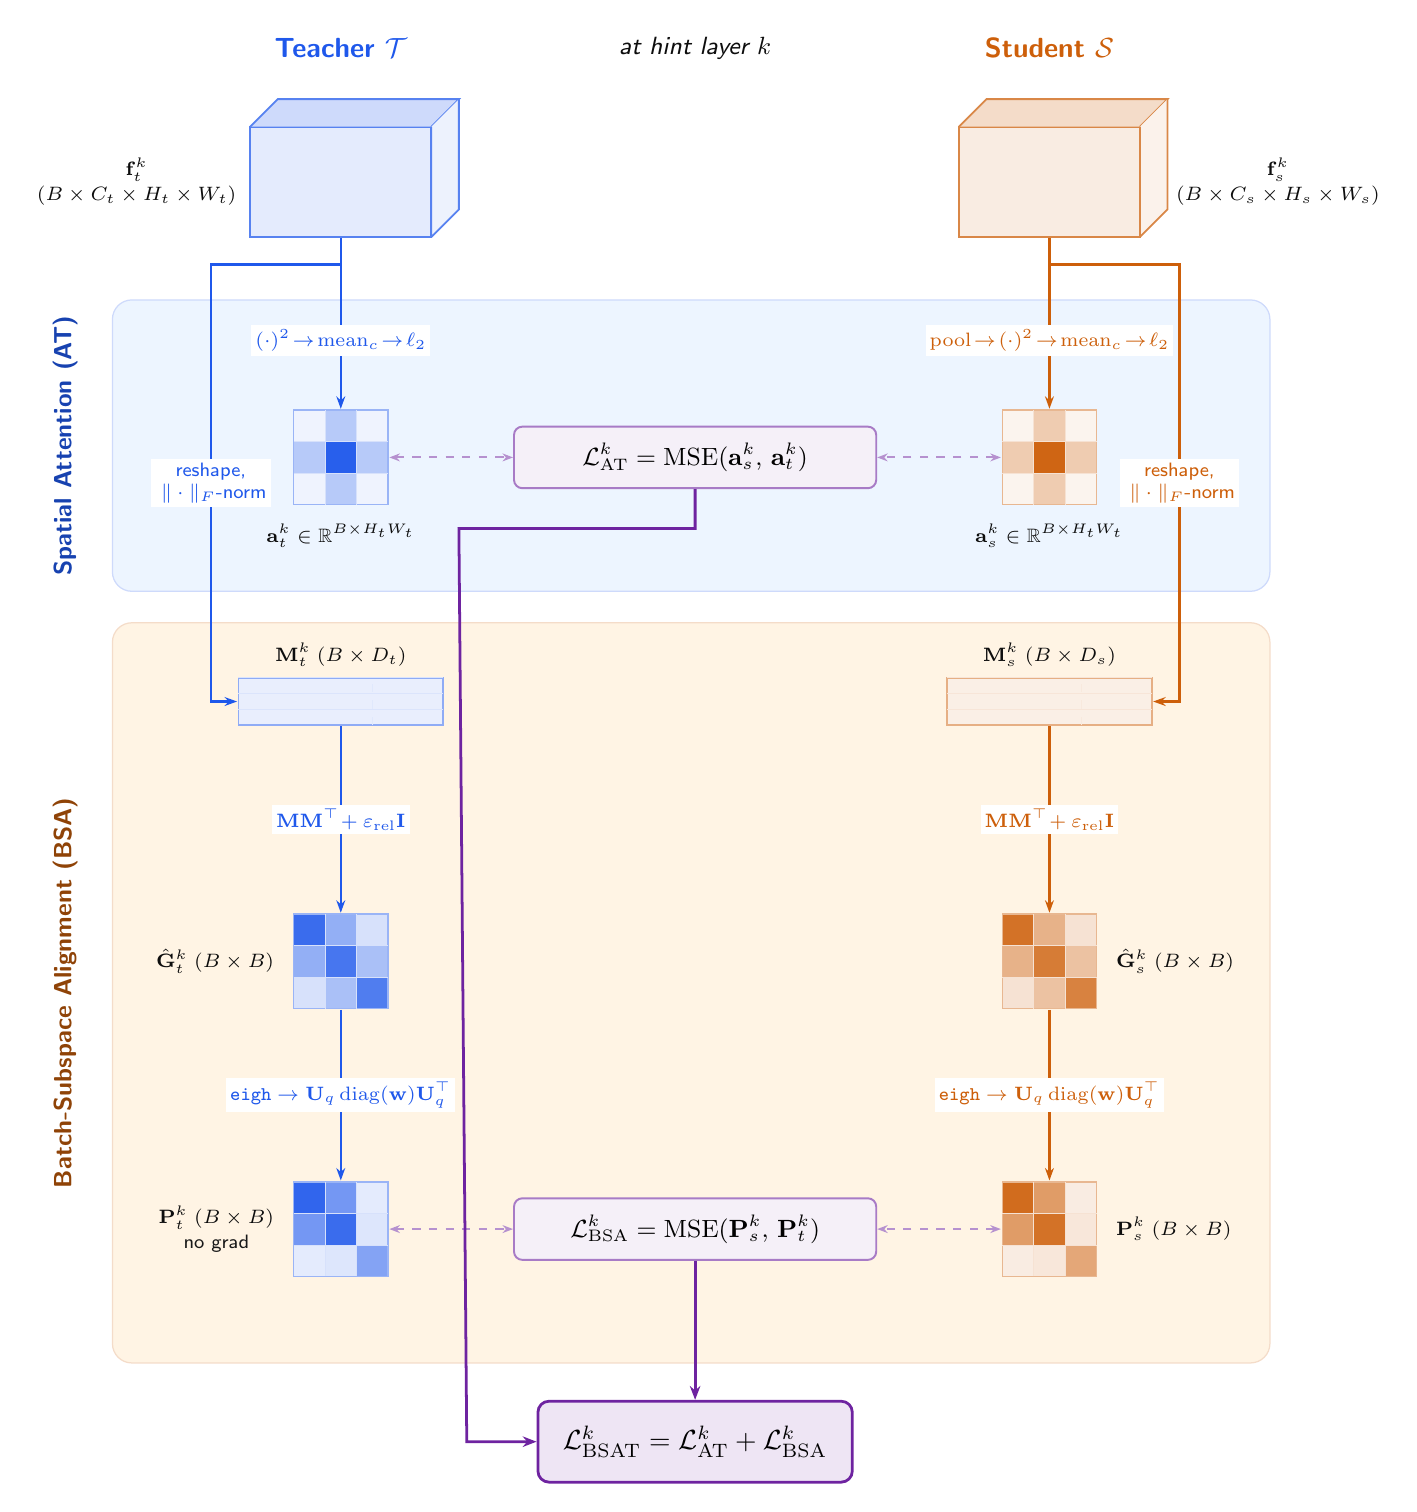
\begin{tikzpicture}[
  font=\small\sffamily,
  %% inline arrow label: white fill only, no border
  lbl/.style={font=\scriptsize\sffamily, fill=white,
              inner sep=1.5pt, align=center},
  %% MSE / loss formula box
  bm/.style={draw=Cm!60, line width=0.7pt, fill=Cm!7,
             rounded corners=3pt, align=center,
             inner sep=6pt, minimum width=4.6cm},
  %% dim annotation below visual elements
  dlbl/.style={font=\scriptsize\sffamily, text=black!95, align=center},
  At/.style={-{Stealth[length=4.5pt,width=3.2pt]}, line width=0.85pt, Ct},
  As/.style={-{Stealth[length=4.5pt,width=3.2pt]}, line width=0.85pt, Cs},
  Am/.style={-{Stealth[length=5pt,width=3.8pt]},   line width=1.0pt,  Cm},
  Dm/.style={{Stealth[length=3.8pt]}-{Stealth[length=3.8pt]},
             line width=0.75pt, Cm!50, dashed},
]

%% ════════════════════════════════════════════════════════════════════════════
%%  COLUMN HEADERS
%% ════════════════════════════════════════════════════════════════════════════
\node[font=\normalsize\sffamily\bfseries, Ct] at (2.5,  1.7) {Teacher $\mathcal{T}$};
\node[font=\normalsize\sffamily\bfseries, Cs] at (11.5, 1.7) {Student $\mathcal{S}$};
\node[font=\small\sffamily\itshape, black!95]  at (7.0,  1.7) {at hint layer $k$};

%% ════════════════════════════════════════════════════════════════════════════
%%  FEATURE MAPS
%% ════════════════════════════════════════════════════════════════════════════
\fmblock{2.5}{0.0}{Ct}
\node[minimum width=2.32cm,minimum height=1.42cm](ft) at (2.5,0.0){};
\node[dlbl,left=1pt of ft]{$\mathbf{f}_t^k$\\[1pt]$(B\times C_t\times H_t\times W_t)$};

\fmblock{11.5}{0.0}{Cs}
\node[minimum width=2.32cm,minimum height=1.42cm](fs) at (11.5,0.0){};
\node[dlbl,right=9pt of fs]{$\mathbf{f}_s^k$\\[1pt]$(B\times C_s\times H_s\times W_s)$};

%% ════════════════════════════════════════════════════════════════════════════
%%  AT BAND — spatial attention maps
%% ════════════════════════════════════════════════════════════════════════════
\heatmap{2.5}{-3.5}{Ct}{%
  0/0/7,0/1/32,0/2/7,
  1/0/32,1/1/96,1/2/32,
  2/0/7,2/1/32,2/2/7}
\node[minimum width=1.22cm,minimum height=1.22cm](att) at (2.5,-3.5){};
\node[dlbl,below=3pt of att]{$\mathbf{a}_t^k\in\mathbb{R}^{B\times H_tW_t}$};

\heatmap{11.5}{-3.5}{Cs}{%
  0/0/7,0/1/32,0/2/7,
  1/0/32,1/1/96,1/2/32,
  2/0/7,2/1/32,2/2/7}
\node[minimum width=1.22cm,minimum height=1.22cm](ats) at (11.5,-3.5){};
\node[dlbl,below=3pt of ats]{$\mathbf{a}_s^k\in\mathbb{R}^{B\times H_tW_t}$};

\node[bm](mse_at) at (7.0,-3.5)
  {$\mathcal{L}_{\mathrm{AT}}^k =
    \operatorname{MSE}(\mathbf{a}_s^k,\,\mathbf{a}_t^k)$};

\draw[At](ft.south) --
  node[pos=0.6,lbl]{$(\cdot)^2\!\to\!\mathrm{mean}_c\!\to\!\ell_2$} (att.north);
\draw[As](fs.south) --
  node[pos=0.6,lbl]{$\mathrm{pool}\!\to\!(\cdot)^2\!\to\!\mathrm{mean}_c\!\to\!\ell_2$} (ats.north);
\draw[Dm](att.east) -- (mse_at.west);
\draw[Dm](ats.west) -- (mse_at.east);

%% ════════════════════════════════════════════════════════════════════════════
%%  BSA BAND — flatten → Gram → projector
%% ════════════════════════════════════════════════════════════════════════════

%% M matrices (B×D)
\mmatrix{2.5}{-6.6}{Ct}
\node[minimum width=2.62cm,minimum height=0.62cm](Mt) at (2.5,-6.6){};
\node[dlbl,above=0pt of Mt]{$\mathbf{M}_t^k\;(B\times D_t)$};

\mmatrix{11.5}{-6.6}{Cs}
\node[minimum width=2.62cm,minimum height=0.62cm](Ms) at (11.5,-6.6){};
\node[dlbl,above=0pt of Ms]{$\mathbf{M}_s^k\;(B\times D_s)$};

%% BSA outer-margin arrows (placed here so Mt and Ms are already defined)
\draw[At](ft.south) -- (2.5,-1.05) -- (0.85,-1.05)
  -- node[pos=0,lbl,midway]{reshape,\\\;$\|\cdot\|_F$-norm}
  (0.85,-6.60) -- (Mt.west);
\draw[As](fs.south) -- (11.5,-1.05) -- (13.15,-1.05)
  -- node[pos=0,lbl,midway]{reshape,\\\;$\|\cdot\|_F$-norm}
  (13.15,-6.60) -- (Ms.east);

%% Gram matrices (B×B)
\heatmap{2.5}{-9.9}{Ct}{%
  0/0/88,0/1/48,0/2/18,
  1/0/48,1/1/82,1/2/38,
  2/0/18,2/1/38,2/2/78}
\node[minimum width=1.22cm,minimum height=1.22cm](Gt) at (2.5,-9.9){};
\node[dlbl,left=3pt of Gt]{$\hat{\mathbf{G}}_t^k\;(B\times B)$};

\heatmap{11.5}{-9.9}{Cs}{%
  0/0/88,0/1/48,0/2/18,
  1/0/48,1/1/82,1/2/38,
  2/0/18,2/1/38,2/2/78}
\node[minimum width=1.22cm,minimum height=1.22cm](Gs) at (11.5,-9.9){};
\node[dlbl,right=3pt of Gs]{$\hat{\mathbf{G}}_s^k\;(B\times B)$};

%% Projectors (B×B)
\heatmap{2.5}{-13.3}{Ct}{%
  0/0/92,0/1/62,0/2/12,
  1/0/62,1/1/88,1/2/15,
  2/0/12,2/1/15,2/2/55}
\node[minimum width=1.22cm,minimum height=1.22cm](Pt) at (2.5,-13.3){};
\node[dlbl,left=3pt of Pt]{%
  $\mathbf{P}_t^k\;(B\times B)$\\[1pt]{\color{black!90}\scriptsize no grad}};

\heatmap{11.5}{-13.3}{Cs}{%
  0/0/92,0/1/62,0/2/12,
  1/0/62,1/1/88,1/2/15,
  2/0/12,2/1/15,2/2/55}
\node[minimum width=1.22cm,minimum height=1.22cm](Ps) at (11.5,-13.3){};
\node[dlbl,right=3pt of Ps]{$\mathbf{P}_s^k\;(B\times B)$};

\node[bm](mse_bsa) at (7.0,-13.3)
  {$\mathcal{L}_{\mathrm{BSA}}^k =
    \operatorname{MSE}(\mathbf{P}_s^k,\,\mathbf{P}_t^k)$};

%% (BSA arrows come from feature maps via outer margin — see above)

\draw[At](Mt.south) --
  node[pos=0,lbl,midway]{$\mathbf{M}\mathbf{M}^\top\!+\varepsilon_\mathrm{rel}\mathbf{I}$} (Gt.north);
\draw[As](Ms.south) --
  node[pos=0,lbl,midway]{$\mathbf{M}\mathbf{M}^\top\!+\varepsilon_\mathrm{rel}\mathbf{I}$} (Gs.north);

\draw[At](Gt.south) --
  node[pos=0,lbl,midway]{\texttt{eigh}\;$\to\mathbf{U}_q\operatorname{diag}(\mathbf{w})\mathbf{U}_q^\top$} (Pt.north);
\draw[As](Gs.south) --
  node[pos=0,lbl,midway]{\texttt{eigh}\;$\to\mathbf{U}_q\operatorname{diag}(\mathbf{w})\mathbf{U}_q^\top$} (Ps.north);

\draw[Dm](Pt.east) -- (mse_bsa.west);
\draw[Dm](Ps.west) -- (mse_bsa.east);

%% ════════════════════════════════════════════════════════════════════════════
%%  FINAL LOSS
%% ════════════════════════════════════════════════════════════════════════════
\node[draw=Cm, line width=1.0pt, fill=Cm!12, rounded corners=4pt,
      align=center, inner sep=9pt, font=\normalsize\sffamily]
  (loss) at (7.0,-16.0)
  {$\mathcal{L}_{\mathrm{BSAT}}^k =
    \mathcal{L}_{\mathrm{AT}}^k + \mathcal{L}_{\mathrm{BSA}}^k$};

%% mse_at → loss  (route left of mse_bsa)
\draw[Am](mse_at.south) -- ++(0,-0.50)
  -- ++(-3.0,0.0) -- (4.1,-16) -- (loss.west);
%% mse_bsa → loss  (direct)
\draw[Am](mse_bsa.south) -- (loss.north);

%% ════════════════════════════════════════════════════════════════════════════
%%  BAND BACKGROUNDS
%% ════════════════════════════════════════════════════════════════════════════
\begin{pgfonlayer}{background}
  \fill[Cbgat, rounded corners=7pt]
    (-0.4,-1.5) rectangle (14.3,-5.2);
  \draw[Ct!22, rounded corners=7pt, line width=0.45pt]
    (-0.4,-1.5) rectangle (14.3,-5.2);
  \fill[Cbgbsa, rounded corners=7pt]
    (-0.4,-5.6) rectangle (14.3,-15.0);
  \draw[Cs!22, rounded corners=7pt, line width=0.45pt]
    (-0.4,-5.6) rectangle (14.3,-15.0);
\end{pgfonlayer}

%% band labels
\node[rotate=90,font=\small\sffamily\bfseries,text=Ct!75!black]
  at (-1.0,-3.35) {Spatial Attention (AT)};
\node[rotate=90,font=\small\sffamily\bfseries,text=Cs!70!black]
  at (-1.0,-10.30) {Batch-Subspace Alignment (BSA)};

\end{tikzpicture}
\end{document}
